\section{简谐振动的合成}\label{sec:07.06}

简谐振动只是振动或周期运动中的一种,许多实际的周期运
\clearpage
% 214.jpg
\noindent 动并不是简谐的。例如,各种乐器的振动大都不是简谐振动。所
谓音色,就是决定于振动的形式。譬如,小提琴的振动有如图
\ref{fig:07.10}\;所示的锯齿形。各种乐器都有自己的独特振动形式。

\begin{figurex}
  \centering
  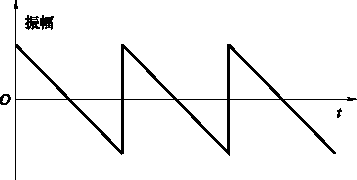
\includegraphics{figure/fig07.10}
  \caption{小提琴的振动}
  \label{fig:07.10}
\end{figurex}
\vspace{0.5em}

这种情况,似乎要求我们把振动按其形式分为多种类型来建
立理论。其实不然,因为各种周期振动都可以由简谐振动组成。
理论上可以证明:任意一个周期振动$ x = f \left( t \right) $,即$ f \left( t \right) $是$ t $的周期
函数,以$ T $为周期,即
\begin{equation}\label{eqn:07.06.01}
  f \left( t + n T \right) = f ( t )
\end{equation}
其中$ n $为任意正、负整数,则$ f \left( t \right) $可以表示成
{\setlength{\mathindent}{4em}
\begin{equation}\label{eqn:07.06.02}
  \begin{aligned}
    f \left( t \right) = & A _ { 0 } + A _ { 1 } \cos \left( \omega t + \varphi _ { 1 } \right) + A _ { 2 } \cos \left( 2 \omega t + \varphi _ { 2 } \right) \\
                         & + A _ { 3 } \cos \left( 3 \omega t + \varphi _ { 3 } \right) + \cdots
  \end{aligned}
\end{equation}}
其中$\omega = \dfrac { 2 \uppi } { T } $;$ A _ { 0 }, A _ { 1 }, A _ { 2 }, \dots $决定于$ f \left( t \right) $的具体形式。式\eqref{eqn:07.06.01}
及式\eqref{eqn:07.06.02}表示,任何一个周期为$ T $的振动,可以看成是由周期
为$ T, \dfrac { 1 } { 2 } T , \dfrac { 1 } { 3 } T  , \dots $一系列简谐振动相加而成的。例如上述小
提琴的振动可写为
\begin{equation*}
  x = A \left( \sin \omega t + \frac { 1 } { 2 } \sin 2 \omega t + \frac { 1 } { 3 } \sin 3 \omega t + \cdots \right)
\end{equation*}
所谓音色,就决定于$ A _ { 1 } , A _ { 2 }, \dots $各项简谐振动的振幅之比例。声
% 215.jpg
音是否和谐,也就决定于这些比例。小提琴的一系列振幅的比是
$ \dfrac { 1 } { 1 } : \dfrac { 1 } { 2 } : \dfrac { 1 } { 3 }
  : \cdots $非常简单而有规律,这就是小提琴声音优美动听的
物理原因。

现在讨论几种简单的振动合成问题。

(1)一种最简单的情况是
\begin{equation}\label{eqn:07.06.03}
  x = A _ { 1 } \cos \left( \omega t + \varphi _ { 1 } \right) + A _ { 2 } \cos \left( \omega t + \varphi _ { 2 } \right)
\end{equation}
这表示质点的运动是两种简谐振动合成的结果,而且这两种简谐
振动具有相同的周期。

利用三角公式,可以将上式改写成
\begin{equation}\label{eqn:07.06.04}
  \begin{aligned}
    x = & \left( A _ { 1 } \cos \varphi _ { 1 } + A _ { 2 } \cos \varphi _ { 2 } \right) \cos \omega t   \\[-0.5em]
        & - \left( A _ { 1 } \sin \varphi _ { 1 } + A _ { 2 } \sin \varphi _ { 2 } \right) \sin \omega t
  \end{aligned}
\end{equation}
令\vspace{-1.56em}
\begin{equation}\label{eqn:07.06.05}
  \begin{aligned}
    A _ { 1 } \cos \varphi _ { 1 } + A _ { 2 } \cos \varphi _ { 2 }  & = A  \cos \varphi \\[-0.5em]
    A _ { 1 } \sin \varphi _ { 1 } + A _ { 2 }  \sin \varphi _ { 2 } & = A  \sin \varphi
  \end{aligned}
\end{equation}
则式\eqref{eqn:07.06.04}成为
\begin{equation}\label{eqn:07.06.06}
  x = A  \cos \left( \omega t +  \varphi \right)
\end{equation}
由式\ref{eqn:07.06.05},$ A $及$ \varphi $可以表示成
\begin{equation}\label{eqn:07.06.07}
  \begin{split}
    A &= \sqrt { A _ { 1 } ^ { 2 } + A _ 2 ^ { 2 } + 2 A _ { 1 } A _ { 2 }  \cos \left( \varphi _ { 1 } -  \varphi _ { 2 } \right) } \\
    \tg \varphi &= \frac { A _ { 1 }  \sin \varphi _ { 1 } + A _ { 2 } \sin \varphi _ { 2 } } { A _ { 1 }  \cos \varphi _ { 1 } + A _ { 2 } \cos \varphi _ { 2 } }
  \end{split}
\end{equation}
式\eqref{eqn:07.06.06}表示,两个相同周期(或频率)的简谐振动合成的结果
\begin{wrapfigure}[7]{r}{13em}
  \vspace{-1em}
  \centering
  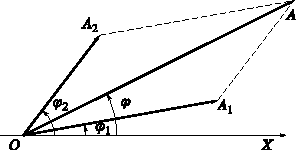
\includegraphics{figure/fig07.11}
  \caption{振动的合成}
  \label{fig:07.11}
\end{wrapfigure}
仍是一个简谐振动,并具有相同周期,只是振幅和位相
应取式\eqref{eqn:07.06.07}给出的值。

式\eqref{eqn:07.06.07}也很容易由几何方法得到。按\ref{sec:07.03}节的方法,每个简谐振动可用一
矢量表示,则式\eqref{eqn:07.06.03}应由
% 216.jpg
图\ref{fig:07.11}\;中的矢量$ \vec{OA_1} $及$ \vec{OA_2} $表示。由于$ \vec{ O A _ { 1 } } , \vec{ O A _ { 2 } } $绕$ O $转动的角速
度(即$ \omega $)相同,所以二者相对位相不变,因此二者在$ OX $方向的
投影之和,就等于矢量$\vec{OA}$的投影。$ \vec{OA} $为$\vec{OA_1}$及$\vec{OA_2}$的矢量和。
由$  A _ { 1 }   ,  A _ { 2 }  ,\varphi_{ 1 },\varphi_{ 2 }$可求出$ A $及$\varphi$,结果仍然是式\eqref{eqn:07.06.07}。

(2)两个振幅相同,但周期差别很小的简谐振动的合成,即
\begin{equation}\label{eqn:07.06.08}
  x = A \cos \left( \omega _ { 1 } t + \varphi \right) + A  \cos \left( \omega _ { 2 } t + \varphi \right)
\end{equation}
其中$\omega_{ 1 }$与$\omega_{ 2 }$的差很小。
\begin{equation*}
  \left| \omega _ { 1 } - \omega _ { 2 } \right| \ll \omega _ { 1 } , \omega _ { 2 }
\end{equation*}
利用三角公式,式\eqref{eqn:07.06.08}可以改写成
\begin{equation*}
  \begin{split}
    x &= 2 A  \cos \left( \frac { \omega _ { 1 } - \omega _ { 2 } } { 2 } t \right)  \cos \left( \frac { \omega _ { 1 } + \omega _ { 2 } t } { 2 } t  + \varphi \right)  \\
    & \approx 2 A  \cos \left( \frac { \omega _ { 1 } - \omega _ { 2 } } { 2 } t \right)  \cos \left( \omega _ { 1 } t + \varphi \right)
  \end{split}
\end{equation*}
这个公式的物理意义是,质点仍作频率为$\omega_{ 1 }$的简谐振动,但它的
振幅不是常数,而是$ \left| 2 A  \cos \dfrac { \omega _ { 1 } - \omega _ { 2 } } { 2 } t \right| $,即振幅也是随时间周期
变化的。振幅的平方正比于振动能量,所以,这种振动具有周期
生的强弱变化,这种现象称为拍。振幅的变化周期即为拍的周期。
由于振幅只涉及$ \cos \dfrac { \omega _ { 1 } - \omega _ { 2 } } { 2 } t $的绝对值,所以,单位时间中的振
福变化次数等于的$ \dfrac { 1 } { 2 \uppi } - \dfrac { \left| \omega _ { 1 } - \omega _ { 2 } \right| } { 2 } $两倍,故拍的周期为
\begin{equation*}
  T _ { \text { 拍 } } = \frac { 2 \uppi } { \left| \omega _ { 1 } - \omega _ { 2 } \right| }
\end{equation*}

(3)二维的振动合成。由\ref{sec:07.03}节的讨论已知,一个匀速圆周运
力可以看成在$ X $,$ Y $两个方向上的简谐振动的合成,即匀速圆周
运动可表示为
% 217.jpg
\begin{equation}\label{eqn:07.06.09}
  \begin{cases}
    x = r _ { 0 } \cos \left( \omega t + \varphi _ { 0 } \right) \\
    y = r _ { 0 } \sin \left( \omega t + \varphi _ { 0 } \right)
  \end{cases}
\end{equation}
其中$ r _ { 0 } $为圆周的半径。

现在我们把式\eqref{eqn:07.06.09}加以推广。假定$ x $方向与$ y $方向振动的
位相不一定相同,即
\begin{equation}\label{eqn:07.06.10}
  \begin{cases}
    x = r _ { 0 } \cos \left( \omega t + \varphi _ { 1 } \right) \\
    y = r _ { 0 } \sin \left( \omega t + \varphi _ { 2 } \right)
  \end{cases}
\end{equation}
这时,运动的形态完全取决于$  \varphi _ { 1 }   $, $ \varphi _ { 2 }   $的相互关系。

如果$  \varphi _ { 2 } - \varphi _ { 1 } = 3 \uppi / 2 $,则式\eqref{eqn:07.06.10}变为式\eqref{eqn:07.06.09},它是匀速
圆周运动。

如果$   \varphi _ { 2 } - \varphi _ { 1 } = 0  $ ,则式\eqref{eqn:07.06.10}成为
\begin{equation*}
  \begin{split}
    x = r _ { 0 }  \cos \left( \omega t + \varphi _ { 1 } \right)  \\[-0.5em]
    y = r _ { 0 }  \cos \left( \omega t + \varphi _ { 1 } \right)
  \end{split}
\end{equation*}
因此,这时的轨迹是一段直线:
\begin{equation*}
  x = y \quad \left| x \right| , \left| y \right| \leqslant r _ { 0 }
\end{equation*}\label{err:07.06.01}
如果定义坐标
\begin{equation*}
  r = \sqrt { x ^ { 2 } + y ^ { 2 } }
\end{equation*}
则\vspace{-1.56em}
\begin{equation*}
  r = \sqrt { 2 } r _ { 0 }  \cos \left( \omega t +  \varphi _ { 1 } \right)
\end{equation*}
故质点是沿着图712(a)的斜线方向作简谐振动。

为了讨论一般情况,我们可以从式\eqref{eqn:07.06.10}得出
\begin{equation}\label{eqn:07.06.11}
  \begin{split}
    x + y &= r _ { 0 }  \cos \left( \omega t + \varphi _ { 1 } \right) + r _ { 0 }  \cos \left( \omega t +  \varphi _ { 2 } \right)  \\[-0.5em]
    &= A _ { + }  \cos \left( \omega t + \varphi \right) \\[-0.5em]
    x - y &= r _ { 0 }  \cos \left( \omega t +  \varphi _ { 1 } \right) - r _ { 0 }  \cos \left( \omega t +  \varphi _ { 2 } \right)  \\[-0.5em]
    &= A _ { - }  \sin \left( \omega t + \varphi \right)
  \end{split}
\end{equation}
其中\vspace{-1.56em}
\begin{equation}\label{eqn:07.06.12}
  \begin{split}
    A _ { + } &= \sqrt { 2 } r _ { 0 } \sqrt { 1 + \cos \left( \varphi _ { 1 } -  \varphi _ { 2 } \right) }  \\[-0.5em]
    A _ { - } &= \sqrt { 2 } r _ { 0 } \sqrt { 1 - \cos \left( \varphi _ { 1 } -  \varphi _ { 2 } \right) } \\[-0.5em]
    \tg \varphi &= \frac { \sin \varphi _ { 1 } + \sin \varphi _ { 2 } } { \cos \varphi _ { 1 } + \cos \varphi _ { 2 } }
  \end{split}
\end{equation}
% 218.jpg
由式\eqref{eqn:07.06.11}即得
\begin{equation*}
  \frac { \left( x + y \right) ^ { 2 } } { A _ { + } ^ { 2 } } + \frac { \left( x - y \right) ^ { 2 } } { A _ { - } ^ { 2 } } = 1
\end{equation*}
可见,式\eqref{eqn:07.06.10}表示的运动轨迹,一般情况是一个椭圆。椭圆
的长轴或短轴沿着$ \pm 45 ^ { \circ } $线,两轴长分别为$ A _ { + } $及$ A _ { - } $。由此,不难
从位相差$ \varphi_{ 2 } - \varphi_{ 1 } $给出一系列不同的运动形态(图\ref{fig:07.12})。\vspace{1.56em}
\begin{figurex}
  \centering
  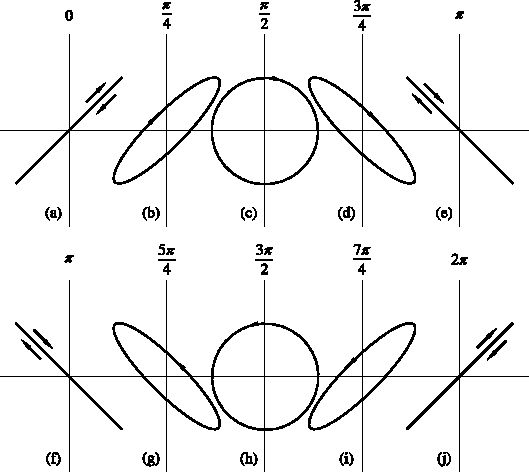
\includegraphics{figure/fig07.12}
  \caption{二维振动的合成}
  \label{fig:07.12}
\end{figurex}
